\section{Implementation and information access}\label{app:implementation}

\paragraph{Physical model.}
The packed state is $(h_1,h_2,h_3,T_{m1},T_{m2},T_{m3},r_b,m_{\ell1},m_{\ell2},
d_{sw1},d_{sw2})$. Temperature--enthalpy relations use a tabulated IAPWS
property grid. The observation map reads physical states and supplied boundaries;
there is no separate neural mean-temperature head. The steady anchor uses
physical observation inversion. The hybrid corrects only metal temperatures
and fuel lag; all three steam enthalpies and both liquid/transport pairs retain
their anchored initial values. Mean corrections are bounded by 0.1 times fixed
state scales. Zero-initialized observer heads return the anchor exactly.
Five 2\,s substeps form one 10\,s sample step. The closure is recomputed at the
current state of each substep; Equation~\ref{eq:trans} abbreviates this composition.

\paragraph{Closure restrictions.}
A two-hidden-layer tanh MLP returns three bounded power corrections, one per
segment. The conservative mode applies equal and opposite steam/metal injections.
Inputs are normalized physical state and six allowed base boundaries, excluding
measured total spray. There are no additional latent dimensions or stochastic
closure inputs in this round. Input exclusion is a direct-interface property:
states already depend on earlier actions. With $S_k=\partial x_k/\partial\epsilon$
under an action perturbation, the local chain rule includes
\[
S_{k+1}=(\Phi_x+\Phi_r r_x)S_k+\Phi_u\,
\frac{\partial u_{k+1}}{\partial\epsilon},\qquad S_t=0.
\]
Thus the learned closure can still modify sensitivities through the state.
The opposite injections constrain where residual heat enters, but do not prove
parameter identifiability, numerical stability in every regime, or true gain recovery.

\paragraph{Observer candidate.}
Both hybrid observers have hidden width 128. The candidate patches each of 23
historical variables with patch length 16 and stride 8 (11 patches per variable,
253 tokens). Linear patch embeddings plus variable and patch embeddings enter
one four-head Transformer encoder; 11 learned state queries cross-attend to
its output. Per-state correction heads receive the query features and pressure
features. The GRU and candidate share the correction bound, state mask,
physical transition, closure, historical extensions and seed-specific training
draws. The token candidate uses no future-history tokens. This is an observer
replacement, not an end-to-end replacement of physical dynamics by attention.

\paragraph{Black box.}
Inspired by variable-token forecasting~\cite{liu2024itransformer}, a linear
96-to-64 projection embeds each of 23 historical channels. A separate 18-to-64
projection embeds each of nine supplied future channels (two valves, seven
base boundaries). Two four-head Transformer layers process the 32 tokens;
a flattened linear head predicts 18 main-steam deviations from the historical
main-steam mean. Dropout is 0.1 and feedforward width is 128. This local adapted
baseline should not be confused with a reproduction of the original benchmark
architecture or the physics-guided steam-temperature predictor~\cite{zhang2026sst}.

\begin{table}[!ht]
\centering\small
\begin{tabular}{lrrrr}
\toprule
Property & Black box & Grey box & Hybrid GRU & Hybrid token\\
\midrule
Historical extensions consumed & 9 & 0 & 9 & 9\\
Learned observer & --- & --- & GRU & Patch/query\\
Neural power closure & --- & None & Conservative & Conservative\\
Rewetting & --- & Enabled & Ablated & Ablated\\
Parameters receiving gradients & 111,250 & 99 & 65,808 & 278,248\\
Update cap & 3,000 & 24,000 & 24,000 & 24,000\\
Batch size & 128 & 32 & 32 & 32\\
Validation frequency (updates) & 500 & 200 & 200 & 200\\
Patience (evaluations) & 3 & 20 & 20 & 20\\
\bottomrule
\end{tabular}
\caption{Executed configuration, not a capacity- or compute-matched benchmark.
Active counts exclude instantiated but bypassed networks. In structured models,
observation uncertainty parameters can receive gradients through NLL.}
\end{table}

\section{Data contract, estimator and provenance}\label{app:stats}

The seven base channels are steam flow, coal command, separator pressure,
separator temperature, feedwater temperature, outlet pressure and total spray
flow. The nine extensions are corrected fuel, active mill count, weighted mill
gas temperature, flue oxygen, total secondary air, reheater gas inlet temperatures
A/B, water--coal ratio and unit load. They inform history only: no recorded
future extension is passed into any arm. Water--coal ratio is a covariate, not
an additional physical power correction. Its isolated benefit is not identified
without a feature ablation.

The physical model uses fixed engineering scales for base channels. Extensions
use shared training-only means and standard deviations. The black box uses
training-only statistics for all historical channels and the historical target
mean for its output offset; its supplied future base covariates are not normalized
by that historical transform. Future total spray is visible to the black box but
ignored by action-driven physics. Holding it fixed during a valve change defines
the diagnostic input, not a self-consistent plant counterfactual. These details
are reasons to interpret the experiment as a comparison of complete methods.

Training draws use a fixed 20,000-window bank sampled with replacement. Validation
and response manifests use seeds 30,000 and 60,000; the training-bank seed is
15,000. Each training seed controls initialization and subsequent minibatch
draws. All models share identical validation targets, timestamps and starts;
all probes share starts, valve doses and support masks. The prediction set has
256 windows and the probe set 64 histories, each covering 13 UTC days. Overlapping
windows are possible; windows are not treated as independent experimental units.

For each seed, paired H18 error differences are averaged within UTC day.
The 13 daily values are resampled with replacement 1,000 times, RNG seed 11,000;
the 2.5th/97.5th percentiles form the reported interval. The same procedure
applies pointwise to response curves. These intervals quantify day variation
conditional on the selected checkpoints. They are not adjusted for checkpoint
selection, previous validation reuse, multiple comparisons, or cross-day serial
dependence. We do not treat three seeds as independent plants. Figure bands
instead show the min--max range of three seed-level daily means.

\begin{table}[!ht]
\centering\small
\begin{tabular}{lccc}
\toprule
H18 candidate minus reference (\degc{}) & Seed 0 & Seed 1 & Seed 2\\
\midrule
GRU $-$ black box & $0.068$ & $0.046$ & $0.104$\\
95\% day-block interval & $[0.027,0.108]$ & $[-0.002,0.093]$ & $[0.067,0.137]$\\
GRU $-$ grey box & $-0.537$ & $-0.541$ & $-0.500$\\
95\% day-block interval & $[-0.784,-0.318]$ & $[-0.756,-0.341]$ & $[-0.725,-0.299]$\\
Token $-$ GRU & $0.267$ & $0.212$ & $0.154$\\
95\% day-block interval & $[0.210,0.329]$ & $[0.155,0.269]$ & $[0.119,0.193]$\\
\bottomrule
\end{tabular}
\caption{Paired descriptive intervals, independently recalculated from saved arrays.
No selection-adjusted or confirmatory significance claim is made.}
\end{table}

The registered action support check expands each valve's historical marginal
minimum/maximum by 0.05 and checks both base and perturbed sequences. All
64 histories pass for each valve; no history was discarded. This permissive
axis-aligned check does not test joint state--action support, conditional
excitation or the realism of holding all supplied boundaries fixed.
There is therefore no distinct supported-only curve in this round: it would be
identical to the primary curve.

\paragraph{Artifact audit.}
The returned bundle contains 12 checkpoints, training ledgers and 24 raw
prediction/response arrays. A local read-only audit verifies artifact hashes,
checkpoint-to-input-identity binding and common index pairing. An independent
saved-array reduction checks all source fingerprints, recalculates every
prediction curve, response curve and paired interval, and recovers the same
selected hybrid. Input, mapping and thermodynamic-grid fingerprints are retained
in the internal audit record. The execution-side return reports 24 inference
array replays; that statement was not independently rerun from the plant record
in this manuscript-preparation pass. No training or test evaluation was performed
to prepare this draft. The audit verifies the returned evidence, not the
truth of an unmeasured plant intervention response.

\section{Observer selection and per-seed diagnostics}\label{app:ablation}

\begin{figure}[!ht]
\centering
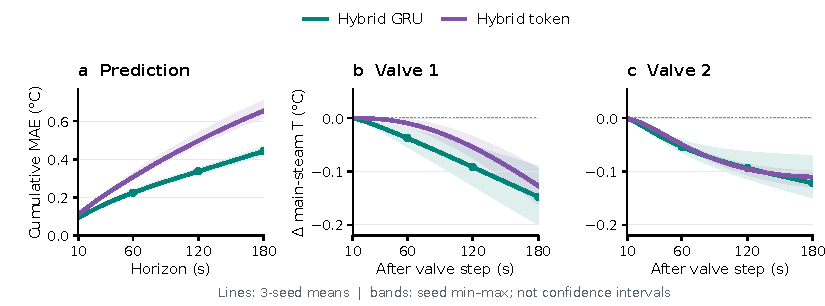
\includegraphics[width=\linewidth]{figures/figS1_observer_ablation_en.pdf}
\caption{\textbf{The token observer does not advance.} Identical physical configuration,
history contract and evaluation manifests; the observer architecture changes.
Token prediction error exceeds GRU at H18 in all seeds, while both have negative
mean endpoint responses. Responses are not model-selection criteria.
Lines and bands use the same definitions as Figure~\ref{fig:evidence}.}
\end{figure}

\begin{table}[!ht]
\centering\small
\begin{tabular}{lrrrr}
\toprule
Method / seed & H18 MAE & Valve 1 H18 & Valve 2 H18 & Best update\\
\midrule
Black box / 0 & 0.3735 & $+0.000013$ & $+0.001335$ & 3,000 \\
Black box / 1 & 0.3756 & $-0.000025$ & $+0.000678$ & 2,500 \\
Black box / 2 & 0.3628 & $+0.000305$ & $+0.000183$ & 3,000 \\
Grey box / 0 & 0.9787 & $+0.004601$ & $+0.032581$ & 23,800 \\
Grey box / 1 & 0.9623 & $+0.004401$ & $+0.033384$ & 24,000 \\
Grey box / 2 & 0.9668 & $+0.004435$ & $+0.033175$ & 24,000 \\
Hybrid GRU / 0 & 0.4414 & $-0.198801$ & $-0.145255$ & 21,000 \\
Hybrid GRU / 1 & 0.4216 & $-0.090115$ & $-0.070247$ & 23,600 \\
Hybrid GRU / 2 & 0.4664 & $-0.152901$ & $-0.149205$ & 21,000 \\
Hybrid token / 0 & 0.7086 & $-0.161024$ & $-0.099171$ & 23,800 \\
Hybrid token / 1 & 0.6340 & $-0.094119$ & $-0.128567$ & 23,600 \\
Hybrid token / 2 & 0.6203 & $-0.125057$ & $-0.102259$ & 22,000 \\
\bottomrule
\end{tabular}

\caption{Seed-level daily means in \degc{}; prediction is cumulative H18 MAE,
response is the H18 endpoint difference, not the last-ten-step metric used in
earlier development. All runs terminate at their caps.}
\label{tab:seeds}
\end{table}

For GRU, the valve-1 endpoint intervals for seeds 0/1/2 are respectively
$[-0.229,-0.167]$, $[-0.105,-0.075]$, $[-0.176,-0.128]$\degc{};
valve-2 intervals are $[-0.168,-0.119]$, $[-0.083,-0.057]$, and
$[-0.172,-0.123]$\degc{}. They support a negative model response under this
probe. Small black-box differences are close to the numerical granularity of
large absolute-temperature predictions; we neither equate them with exactly
zero nor interpret a ratio to them as a physical amplification factor.

\section{Design history and remaining evidence boundaries}

Earlier development investigated initial-state flexibility, residual placement,
boundary prediction and rewetting diagnostics. Those comparisons used different
output aggregations or information contracts; their MAEs are not pooled with
the present main-steam-only metric. They motivated the anchored hybrid and
no-rewetting candidate, but are not confirmatory replications of this new
comparison. In particular, a prior five-temperature average and a current
main-steam-only average are not interchangeable, and earlier H60 probes do not
extend the present registered 180\,s evidence.

The remaining questions require different evidence. A one-time locked-test
evaluation can address temporal generalization after selection, but not true
intervention gains. A matched grey-box no-rewetting comparison would isolate
the effect of adding the observer/closure more cleanly than the present
cross-family contrast. Independently calibrated intervention or suitably
identified natural-experiment responses would address plant-response magnitude.
History-only prediction with forecast rather than recorded future boundaries
would address prospective use. After examining the present results, the
no-rewetting grey-box control has been separately registered with three seeds
and the original budget; it remains pending. Other checks remain proposals,
not completed results or silent changes to the existing protocol.

\paragraph{Data availability and anonymization.}
The data describe an operating industrial process. Public release authorization
for raw plant records has not been established; this draft makes no promise of
open raw data. Numerical figure sources, experiment configuration and audit
records exist locally. An anonymous sharing package and its permissions must
be confirmed before submission; private repository links and site identity are
not included here.

\paragraph{Use of language-model assistance.}
Language-model tools assisted manuscript organization, translation, figure-script
development and consistency checks against saved results. They were not used as
a substitute for plant-response measurements. Human authors remain responsible
for the final scientific claims, numerical verification and submission.
